
\documentclass{article} % For LaTeX2e
\usepackage{iclr2024_conference,times}
\usepackage{graphicx}

% Optional math commands from https://github.com/goodfeli/dlbook_notation.
%%%%% NEW MATH DEFINITIONS %%%%%

\usepackage{amsmath,amsfonts,bm}

% Mark sections of captions for referring to divisions of figures
\newcommand{\figleft}{{\em (Left)}}
\newcommand{\figcenter}{{\em (Center)}}
\newcommand{\figright}{{\em (Right)}}
\newcommand{\figtop}{{\em (Top)}}
\newcommand{\figbottom}{{\em (Bottom)}}
\newcommand{\captiona}{{\em (a)}}
\newcommand{\captionb}{{\em (b)}}
\newcommand{\captionc}{{\em (c)}}
\newcommand{\captiond}{{\em (d)}}

% Highlight a newly defined term
\newcommand{\newterm}[1]{{\bf #1}}


% Figure reference, lower-case.
\def\figref#1{figure~\ref{#1}}
% Figure reference, capital. For start of sentence
\def\Figref#1{Figure~\ref{#1}}
\def\twofigref#1#2{figures \ref{#1} and \ref{#2}}
\def\quadfigref#1#2#3#4{figures \ref{#1}, \ref{#2}, \ref{#3} and \ref{#4}}
% Section reference, lower-case.
\def\secref#1{section~\ref{#1}}
% Section reference, capital.
\def\Secref#1{Section~\ref{#1}}
% Reference to two sections.
\def\twosecrefs#1#2{sections \ref{#1} and \ref{#2}}
% Reference to three sections.
\def\secrefs#1#2#3{sections \ref{#1}, \ref{#2} and \ref{#3}}
% Reference to an equation, lower-case.
\def\eqref#1{equation~\ref{#1}}
% Reference to an equation, upper case
\def\Eqref#1{Equation~\ref{#1}}
% A raw reference to an equation---avoid using if possible
\def\plaineqref#1{\ref{#1}}
% Reference to a chapter, lower-case.
\def\chapref#1{chapter~\ref{#1}}
% Reference to an equation, upper case.
\def\Chapref#1{Chapter~\ref{#1}}
% Reference to a range of chapters
\def\rangechapref#1#2{chapters\ref{#1}--\ref{#2}}
% Reference to an algorithm, lower-case.
\def\algref#1{algorithm~\ref{#1}}
% Reference to an algorithm, upper case.
\def\Algref#1{Algorithm~\ref{#1}}
\def\twoalgref#1#2{algorithms \ref{#1} and \ref{#2}}
\def\Twoalgref#1#2{Algorithms \ref{#1} and \ref{#2}}
% Reference to a part, lower case
\def\partref#1{part~\ref{#1}}
% Reference to a part, upper case
\def\Partref#1{Part~\ref{#1}}
\def\twopartref#1#2{parts \ref{#1} and \ref{#2}}

\def\ceil#1{\lceil #1 \rceil}
\def\floor#1{\lfloor #1 \rfloor}
\def\1{\bm{1}}
\newcommand{\train}{\mathcal{D}}
\newcommand{\valid}{\mathcal{D_{\mathrm{valid}}}}
\newcommand{\test}{\mathcal{D_{\mathrm{test}}}}

\def\eps{{\epsilon}}


% Random variables
\def\reta{{\textnormal{$\eta$}}}
\def\ra{{\textnormal{a}}}
\def\rb{{\textnormal{b}}}
\def\rc{{\textnormal{c}}}
\def\rd{{\textnormal{d}}}
\def\re{{\textnormal{e}}}
\def\rf{{\textnormal{f}}}
\def\rg{{\textnormal{g}}}
\def\rh{{\textnormal{h}}}
\def\ri{{\textnormal{i}}}
\def\rj{{\textnormal{j}}}
\def\rk{{\textnormal{k}}}
\def\rl{{\textnormal{l}}}
% rm is already a command, just don't name any random variables m
\def\rn{{\textnormal{n}}}
\def\ro{{\textnormal{o}}}
\def\rp{{\textnormal{p}}}
\def\rq{{\textnormal{q}}}
\def\rr{{\textnormal{r}}}
\def\rs{{\textnormal{s}}}
\def\rt{{\textnormal{t}}}
\def\ru{{\textnormal{u}}}
\def\rv{{\textnormal{v}}}
\def\rw{{\textnormal{w}}}
\def\rx{{\textnormal{x}}}
\def\ry{{\textnormal{y}}}
\def\rz{{\textnormal{z}}}

% Random vectors
\def\rvepsilon{{\mathbf{\epsilon}}}
\def\rvtheta{{\mathbf{\theta}}}
\def\rva{{\mathbf{a}}}
\def\rvb{{\mathbf{b}}}
\def\rvc{{\mathbf{c}}}
\def\rvd{{\mathbf{d}}}
\def\rve{{\mathbf{e}}}
\def\rvf{{\mathbf{f}}}
\def\rvg{{\mathbf{g}}}
\def\rvh{{\mathbf{h}}}
\def\rvu{{\mathbf{i}}}
\def\rvj{{\mathbf{j}}}
\def\rvk{{\mathbf{k}}}
\def\rvl{{\mathbf{l}}}
\def\rvm{{\mathbf{m}}}
\def\rvn{{\mathbf{n}}}
\def\rvo{{\mathbf{o}}}
\def\rvp{{\mathbf{p}}}
\def\rvq{{\mathbf{q}}}
\def\rvr{{\mathbf{r}}}
\def\rvs{{\mathbf{s}}}
\def\rvt{{\mathbf{t}}}
\def\rvu{{\mathbf{u}}}
\def\rvv{{\mathbf{v}}}
\def\rvw{{\mathbf{w}}}
\def\rvx{{\mathbf{x}}}
\def\rvy{{\mathbf{y}}}
\def\rvz{{\mathbf{z}}}

% Elements of random vectors
\def\erva{{\textnormal{a}}}
\def\ervb{{\textnormal{b}}}
\def\ervc{{\textnormal{c}}}
\def\ervd{{\textnormal{d}}}
\def\erve{{\textnormal{e}}}
\def\ervf{{\textnormal{f}}}
\def\ervg{{\textnormal{g}}}
\def\ervh{{\textnormal{h}}}
\def\ervi{{\textnormal{i}}}
\def\ervj{{\textnormal{j}}}
\def\ervk{{\textnormal{k}}}
\def\ervl{{\textnormal{l}}}
\def\ervm{{\textnormal{m}}}
\def\ervn{{\textnormal{n}}}
\def\ervo{{\textnormal{o}}}
\def\ervp{{\textnormal{p}}}
\def\ervq{{\textnormal{q}}}
\def\ervr{{\textnormal{r}}}
\def\ervs{{\textnormal{s}}}
\def\ervt{{\textnormal{t}}}
\def\ervu{{\textnormal{u}}}
\def\ervv{{\textnormal{v}}}
\def\ervw{{\textnormal{w}}}
\def\ervx{{\textnormal{x}}}
\def\ervy{{\textnormal{y}}}
\def\ervz{{\textnormal{z}}}

% Random matrices
\def\rmA{{\mathbf{A}}}
\def\rmB{{\mathbf{B}}}
\def\rmC{{\mathbf{C}}}
\def\rmD{{\mathbf{D}}}
\def\rmE{{\mathbf{E}}}
\def\rmF{{\mathbf{F}}}
\def\rmG{{\mathbf{G}}}
\def\rmH{{\mathbf{H}}}
\def\rmI{{\mathbf{I}}}
\def\rmJ{{\mathbf{J}}}
\def\rmK{{\mathbf{K}}}
\def\rmL{{\mathbf{L}}}
\def\rmM{{\mathbf{M}}}
\def\rmN{{\mathbf{N}}}
\def\rmO{{\mathbf{O}}}
\def\rmP{{\mathbf{P}}}
\def\rmQ{{\mathbf{Q}}}
\def\rmR{{\mathbf{R}}}
\def\rmS{{\mathbf{S}}}
\def\rmT{{\mathbf{T}}}
\def\rmU{{\mathbf{U}}}
\def\rmV{{\mathbf{V}}}
\def\rmW{{\mathbf{W}}}
\def\rmX{{\mathbf{X}}}
\def\rmY{{\mathbf{Y}}}
\def\rmZ{{\mathbf{Z}}}

% Elements of random matrices
\def\ermA{{\textnormal{A}}}
\def\ermB{{\textnormal{B}}}
\def\ermC{{\textnormal{C}}}
\def\ermD{{\textnormal{D}}}
\def\ermE{{\textnormal{E}}}
\def\ermF{{\textnormal{F}}}
\def\ermG{{\textnormal{G}}}
\def\ermH{{\textnormal{H}}}
\def\ermI{{\textnormal{I}}}
\def\ermJ{{\textnormal{J}}}
\def\ermK{{\textnormal{K}}}
\def\ermL{{\textnormal{L}}}
\def\ermM{{\textnormal{M}}}
\def\ermN{{\textnormal{N}}}
\def\ermO{{\textnormal{O}}}
\def\ermP{{\textnormal{P}}}
\def\ermQ{{\textnormal{Q}}}
\def\ermR{{\textnormal{R}}}
\def\ermS{{\textnormal{S}}}
\def\ermT{{\textnormal{T}}}
\def\ermU{{\textnormal{U}}}
\def\ermV{{\textnormal{V}}}
\def\ermW{{\textnormal{W}}}
\def\ermX{{\textnormal{X}}}
\def\ermY{{\textnormal{Y}}}
\def\ermZ{{\textnormal{Z}}}

% Vectors
\def\vzero{{\bm{0}}}
\def\vone{{\bm{1}}}
\def\vmu{{\bm{\mu}}}
\def\vtheta{{\bm{\theta}}}
\def\va{{\bm{a}}}
\def\vb{{\bm{b}}}
\def\vc{{\bm{c}}}
\def\vd{{\bm{d}}}
\def\ve{{\bm{e}}}
\def\vf{{\bm{f}}}
\def\vg{{\bm{g}}}
\def\vh{{\bm{h}}}
\def\vi{{\bm{i}}}
\def\vj{{\bm{j}}}
\def\vk{{\bm{k}}}
\def\vl{{\bm{l}}}
\def\vm{{\bm{m}}}
\def\vn{{\bm{n}}}
\def\vo{{\bm{o}}}
\def\vp{{\bm{p}}}
\def\vq{{\bm{q}}}
\def\vr{{\bm{r}}}
\def\vs{{\bm{s}}}
\def\vt{{\bm{t}}}
\def\vu{{\bm{u}}}
\def\vv{{\bm{v}}}
\def\vw{{\bm{w}}}
\def\vx{{\bm{x}}}
\def\vy{{\bm{y}}}
\def\vz{{\bm{z}}}

% Elements of vectors
\def\evalpha{{\alpha}}
\def\evbeta{{\beta}}
\def\evepsilon{{\epsilon}}
\def\evlambda{{\lambda}}
\def\evomega{{\omega}}
\def\evmu{{\mu}}
\def\evpsi{{\psi}}
\def\evsigma{{\sigma}}
\def\evtheta{{\theta}}
\def\eva{{a}}
\def\evb{{b}}
\def\evc{{c}}
\def\evd{{d}}
\def\eve{{e}}
\def\evf{{f}}
\def\evg{{g}}
\def\evh{{h}}
\def\evi{{i}}
\def\evj{{j}}
\def\evk{{k}}
\def\evl{{l}}
\def\evm{{m}}
\def\evn{{n}}
\def\evo{{o}}
\def\evp{{p}}
\def\evq{{q}}
\def\evr{{r}}
\def\evs{{s}}
\def\evt{{t}}
\def\evu{{u}}
\def\evv{{v}}
\def\evw{{w}}
\def\evx{{x}}
\def\evy{{y}}
\def\evz{{z}}

% Matrix
\def\mA{{\bm{A}}}
\def\mB{{\bm{B}}}
\def\mC{{\bm{C}}}
\def\mD{{\bm{D}}}
\def\mE{{\bm{E}}}
\def\mF{{\bm{F}}}
\def\mG{{\bm{G}}}
\def\mH{{\bm{H}}}
\def\mI{{\bm{I}}}
\def\mJ{{\bm{J}}}
\def\mK{{\bm{K}}}
\def\mL{{\bm{L}}}
\def\mM{{\bm{M}}}
\def\mN{{\bm{N}}}
\def\mO{{\bm{O}}}
\def\mP{{\bm{P}}}
\def\mQ{{\bm{Q}}}
\def\mR{{\bm{R}}}
\def\mS{{\bm{S}}}
\def\mT{{\bm{T}}}
\def\mU{{\bm{U}}}
\def\mV{{\bm{V}}}
\def\mW{{\bm{W}}}
\def\mX{{\bm{X}}}
\def\mY{{\bm{Y}}}
\def\mZ{{\bm{Z}}}
\def\mBeta{{\bm{\beta}}}
\def\mPhi{{\bm{\Phi}}}
\def\mLambda{{\bm{\Lambda}}}
\def\mSigma{{\bm{\Sigma}}}

% Tensor
\DeclareMathAlphabet{\mathsfit}{\encodingdefault}{\sfdefault}{m}{sl}
\SetMathAlphabet{\mathsfit}{bold}{\encodingdefault}{\sfdefault}{bx}{n}
\newcommand{\tens}[1]{\bm{\mathsfit{#1}}}
\def\tA{{\tens{A}}}
\def\tB{{\tens{B}}}
\def\tC{{\tens{C}}}
\def\tD{{\tens{D}}}
\def\tE{{\tens{E}}}
\def\tF{{\tens{F}}}
\def\tG{{\tens{G}}}
\def\tH{{\tens{H}}}
\def\tI{{\tens{I}}}
\def\tJ{{\tens{J}}}
\def\tK{{\tens{K}}}
\def\tL{{\tens{L}}}
\def\tM{{\tens{M}}}
\def\tN{{\tens{N}}}
\def\tO{{\tens{O}}}
\def\tP{{\tens{P}}}
\def\tQ{{\tens{Q}}}
\def\tR{{\tens{R}}}
\def\tS{{\tens{S}}}
\def\tT{{\tens{T}}}
\def\tU{{\tens{U}}}
\def\tV{{\tens{V}}}
\def\tW{{\tens{W}}}
\def\tX{{\tens{X}}}
\def\tY{{\tens{Y}}}
\def\tZ{{\tens{Z}}}


% Graph
\def\gA{{\mathcal{A}}}
\def\gB{{\mathcal{B}}}
\def\gC{{\mathcal{C}}}
\def\gD{{\mathcal{D}}}
\def\gE{{\mathcal{E}}}
\def\gF{{\mathcal{F}}}
\def\gG{{\mathcal{G}}}
\def\gH{{\mathcal{H}}}
\def\gI{{\mathcal{I}}}
\def\gJ{{\mathcal{J}}}
\def\gK{{\mathcal{K}}}
\def\gL{{\mathcal{L}}}
\def\gM{{\mathcal{M}}}
\def\gN{{\mathcal{N}}}
\def\gO{{\mathcal{O}}}
\def\gP{{\mathcal{P}}}
\def\gQ{{\mathcal{Q}}}
\def\gR{{\mathcal{R}}}
\def\gS{{\mathcal{S}}}
\def\gT{{\mathcal{T}}}
\def\gU{{\mathcal{U}}}
\def\gV{{\mathcal{V}}}
\def\gW{{\mathcal{W}}}
\def\gX{{\mathcal{X}}}
\def\gY{{\mathcal{Y}}}
\def\gZ{{\mathcal{Z}}}

% Sets
\def\sA{{\mathbb{A}}}
\def\sB{{\mathbb{B}}}
\def\sC{{\mathbb{C}}}
\def\sD{{\mathbb{D}}}
% Don't use a set called E, because this would be the same as our symbol
% for expectation.
\def\sF{{\mathbb{F}}}
\def\sG{{\mathbb{G}}}
\def\sH{{\mathbb{H}}}
\def\sI{{\mathbb{I}}}
\def\sJ{{\mathbb{J}}}
\def\sK{{\mathbb{K}}}
\def\sL{{\mathbb{L}}}
\def\sM{{\mathbb{M}}}
\def\sN{{\mathbb{N}}}
\def\sO{{\mathbb{O}}}
\def\sP{{\mathbb{P}}}
\def\sQ{{\mathbb{Q}}}
\def\sR{{\mathbb{R}}}
\def\sS{{\mathbb{S}}}
\def\sT{{\mathbb{T}}}
\def\sU{{\mathbb{U}}}
\def\sV{{\mathbb{V}}}
\def\sW{{\mathbb{W}}}
\def\sX{{\mathbb{X}}}
\def\sY{{\mathbb{Y}}}
\def\sZ{{\mathbb{Z}}}

% Entries of a matrix
\def\emLambda{{\Lambda}}
\def\emA{{A}}
\def\emB{{B}}
\def\emC{{C}}
\def\emD{{D}}
\def\emE{{E}}
\def\emF{{F}}
\def\emG{{G}}
\def\emH{{H}}
\def\emI{{I}}
\def\emJ{{J}}
\def\emK{{K}}
\def\emL{{L}}
\def\emM{{M}}
\def\emN{{N}}
\def\emO{{O}}
\def\emP{{P}}
\def\emQ{{Q}}
\def\emR{{R}}
\def\emS{{S}}
\def\emT{{T}}
\def\emU{{U}}
\def\emV{{V}}
\def\emW{{W}}
\def\emX{{X}}
\def\emY{{Y}}
\def\emZ{{Z}}
\def\emSigma{{\Sigma}}

% entries of a tensor
% Same font as tensor, without \bm wrapper
\newcommand{\etens}[1]{\mathsfit{#1}}
\def\etLambda{{\etens{\Lambda}}}
\def\etA{{\etens{A}}}
\def\etB{{\etens{B}}}
\def\etC{{\etens{C}}}
\def\etD{{\etens{D}}}
\def\etE{{\etens{E}}}
\def\etF{{\etens{F}}}
\def\etG{{\etens{G}}}
\def\etH{{\etens{H}}}
\def\etI{{\etens{I}}}
\def\etJ{{\etens{J}}}
\def\etK{{\etens{K}}}
\def\etL{{\etens{L}}}
\def\etM{{\etens{M}}}
\def\etN{{\etens{N}}}
\def\etO{{\etens{O}}}
\def\etP{{\etens{P}}}
\def\etQ{{\etens{Q}}}
\def\etR{{\etens{R}}}
\def\etS{{\etens{S}}}
\def\etT{{\etens{T}}}
\def\etU{{\etens{U}}}
\def\etV{{\etens{V}}}
\def\etW{{\etens{W}}}
\def\etX{{\etens{X}}}
\def\etY{{\etens{Y}}}
\def\etZ{{\etens{Z}}}

% The true underlying data generating distribution
\newcommand{\pdata}{p_{\rm{data}}}
% The empirical distribution defined by the training set
\newcommand{\ptrain}{\hat{p}_{\rm{data}}}
\newcommand{\Ptrain}{\hat{P}_{\rm{data}}}
% The model distribution
\newcommand{\pmodel}{p_{\rm{model}}}
\newcommand{\Pmodel}{P_{\rm{model}}}
\newcommand{\ptildemodel}{\tilde{p}_{\rm{model}}}
% Stochastic autoencoder distributions
\newcommand{\pencode}{p_{\rm{encoder}}}
\newcommand{\pdecode}{p_{\rm{decoder}}}
\newcommand{\precons}{p_{\rm{reconstruct}}}

\newcommand{\laplace}{\mathrm{Laplace}} % Laplace distribution

\newcommand{\E}{\mathbb{E}}
\newcommand{\Ls}{\mathcal{L}}
\newcommand{\R}{\mathbb{R}}
\newcommand{\emp}{\tilde{p}}
\newcommand{\lr}{\alpha}
\newcommand{\reg}{\lambda}
\newcommand{\rect}{\mathrm{rectifier}}
\newcommand{\softmax}{\mathrm{softmax}}
\newcommand{\sigmoid}{\sigma}
\newcommand{\softplus}{\zeta}
\newcommand{\KL}{D_{\mathrm{KL}}}
\newcommand{\Var}{\mathrm{Var}}
\newcommand{\standarderror}{\mathrm{SE}}
\newcommand{\Cov}{\mathrm{Cov}}
% Wolfram Mathworld says $L^2$ is for function spaces and $\ell^2$ is for vectors
% But then they seem to use $L^2$ for vectors throughout the site, and so does
% wikipedia.
\newcommand{\normlzero}{L^0}
\newcommand{\normlone}{L^1}
\newcommand{\normltwo}{L^2}
\newcommand{\normlp}{L^p}
\newcommand{\normmax}{L^\infty}

\newcommand{\parents}{Pa} % See usage in notation.tex. Chosen to match Daphne's book.

\DeclareMathOperator*{\argmax}{arg\,max}
\DeclareMathOperator*{\argmin}{arg\,min}

\DeclareMathOperator{\sign}{sign}
\DeclareMathOperator{\Tr}{Tr}
\let\ab\allowbreak


\usepackage{hyperref}
\usepackage{url}


\title{InformatiCup 2024 Ctrl-Alt-Defeat}

% Authors must not appear in the submitted version. They should be hidden
% as long as the \iclrfinalcopy macro remains commented out below.
% Non-anonymous submissions will be rejected without review.

\author{Max Buchholz, Lukas Müller, Levi Otterbach \& Raphael Weber}

% The \author macro works with any number of authors. There are two commands
% used to separate the names and addresses of multiple authors: \And and \AND.
%
% Using \And between authors leaves it to \LaTeX{} to determine where to break
% the lines. Using \AND forces a linebreak at that point. So, if \LaTeX{}
% puts 3 of 4 authors names on the first line, and the last on the second
% line, try using \AND instead of \And before the third author name.

\newcommand{\fix}{\marginpar{FIX}}
\newcommand{\new}{\marginpar{NEW}}

\iclrfinalcopy % Uncomment for camera-ready version, but NOT for submission.
\begin{document}


\maketitle

\begin{abstract}

\end{abstract}

\section{Introduction}
The development of generative Machine Learning models made huge steps forward in the last years considering the comparison with human crafted artefacts. Large Language Models (LLM) enable the generation of texts in all kinds of different flavours and styles. Image generative models like Vision Transformer (ViT) already created fake images being reported as real by media. Other news showed artists winning art competitions with generated art. This creates an interest in detecting which texts or images are AI generated and which ones are real images or human-written texts.

Therefore researchers evaluated different approaches to detect fake images and texts. Some adversarial attacks are already known to be able to reduce the performance of other computer vision tasks, e.g. visual object detection, by artificially manipulating real images.

As this is a very topical issue the "Gesellschaft für Informatik" \cite{GI} organizes a competition called "InformatiCup2024" \cite{InformatiCup} where the participants try to manipulate a detectable source in a way that the detector does not recognize it as AI-generated anymore. This raises the questions, whether and how it is possible to manipulate generated artefacts (e.g. images and texts) to reduce the accuracy of detectors.

It is necessary to evaluate whether such techniques exist, because otherwise one could rely on detectors, which can easily be tricked. If easy efficient manipulation techniques exist, detectors need to be improved or better detectors need to be developed that are robust against these techniques. But this requires a good understanding how the attacks are performed.

Therefore we came up with the following research questions:


RQ1: How can generated images be manipulated to trick fake image detectors?


RQ2: How can generated texts be manipulated to trick fake text generators?


The report is structured as follows: After this introduction chapter 2 presents related work, especially text and image generative models as well as fake image and text detectors. Chapter 3 presents the methodology of our work followed by chapter 4 presenting the results of our experiments. Afterwards the results will be discussed in chapter 5 and chapter 6 will conclude this paper.

\section{Related work}

\subsection{Generative models}

The first image generative model we use is the \textbf{Stable Diffusion} model. It is developed by engineers and researchers from CompVis (\url{https://github.com/CompVis}), Stability AI (\url{https://stability.ai/}) and LAION (\url{https://laion.ai/}) \cite{patil2022stable}. \\
Diffusion models achieve state-of-the-art synthesis results on image data by decomposing the image formation process into sequential applications of denoising autoencoders. Due to its work directly in pixel space, they are very computational expensive. To lower the computational costs, the Stable Diffusion model (v1.5) is applied in a latent space of powerful pretrained autoencoders. This works without losing quality and flexibility. \cite{Rombach_2022_CVPR}

As a second image generative model we use \textbf{OpenDalle} from dataautogpt3 (\url{https://huggingface.co/dataautogpt3/OpenDalle}). OpenDalle, as it is based on the Dall-E model, works by modelling text and image tokens as a single data stream. This is achieved by training a transformer to autoregressively model those tokens into the resulting stream. \\
This is done in two steps:
 
\begin{enumerate}
	\item The images get compressed in a $32 \times 32$ grid of image tokens to reduce the context size of the transformer.
	\item BPE-encoded text tokens are concatenated with the image tokens to model a joint distribution over text and image tokens with the training of an autoregressive transformer.
\end{enumerate}

The exact procedure how DALL-E models work proposed by Ramesh et. al is explained in their paper. \cite{ramesh2021zeroshot}

We choose the \textbf{GPT2} model as one possibility to generate texts for testing our augmentation methods. The GPT model tries to counter the scarcity of labeled text data for machine learning. \\
\cite{radford2018improving} try to avoid this problem in a simple two step procedure:

\begin{enumerate}
	\item A generative pre-training of a language model on a varying corpus of unlabeled text.
	\item Discriminative fine-tuning on every specific task.
\end{enumerate}

To achieve effective transfer with minor changes to the model architecture, task-aware input is used during transformations. \cite{radford2018improving}

The \textbf{Falcon-RW-1B} model built by TII (\url{https://www.tii.ae/}) is the second text generative model we use to test our augmentation models. It is a decoder-only model trained on 350 billion tokens of the RefinedWeb data set. This data set leverages strict filtering and stringent deduplication to uplift the quality of web data. \cite{penedo2023refinedweb}

\subsection{Detector models}

\textbf{Winston AI} is a commercial AI text detector that starts at 18\$ a month. They have two primary methods for checking if a text is AI written. Firstly linguistic analysis analyses every text for characteristics, that are different between human- and AI-generated work. One example characteristic is the repetitiveness, another is Data Training, where the detector saw many AI written texts of one model and learned unique characteristics that this model uses which then can be detected. So this method is more generator-specific. \cite{WinstonAI}

The \textbf{AIorNot} detector by Nahrawy on Hugging Face is a pretrained swin-tiny-patch4-window7-224 fine-tuned on the AI or Not dataset. Swin-Transformer by Microsoft is a new Vision Transformer which makes use of hierarchical windows. This reduces the self-attention to not-overlapping windows of other areas of the image. \cite{liu2021swin}

The \textbf{ai-image-det-resnet18} model is a community made, fine-tuned, resnet18 based, pretrained image detection model. For fine-tuning the author kgmann on Hugging Face used the AI or Not dataset. ResNet-18 is a convolutional neural network that is 18 layers deep. It got pretrained by over a million images from the ImageNet database. \cite{he2015deep}


The \textbf{RoBERTa Base OpenAI Detector} is the output detector model of GPT-2. It was obtained by fine-tuning a RoBERTa base model with the outputs of the GPT-2 model containing 1,5 Billion parameters. The RoBERTa Base OpenAI Detector can be used to classify texts, on whether they are likely to be created by the GPT-2 model. It was published by OpenAI, when the weights of the GPT-2 model 1,5 Billion parameter version was released.

The \textbf{RADAR-Vicuna-7B} text detector is an adversarial-learning trained model introduced by TrustSafeAI. In the training stage a detector tried to differentiate between human and AI text while a paraphraser trained to make the text more human.
The AI-generated text for learning is extracted by the LLM Vicuna-7B-v1.1 written by LMSYS Org \cite{hu2023radar}.


\section{Method}
To test and evaluate the effect of different data augmentation techniques on the detection capabilities of fake image or text detectors, we created a pipeline of three components: The first component is a generator, which is a model capable of generating fake images or texts. The second component is a processor which augments the data through a specified method, after given a generated image or text. The last component is a detector, which suggests an input being either real or fake. This way we can compare it to the ground truth, to evaluate the capabilities of the detector. By comparing the results with augmented artefacts and with the generated ones without augmentation, we can evaluate the effectiveness of different AI detector-tricking techniques.

We used the aforementioned models for generating and detecting texts and images. As for image processors, one was already given in the description of the "InformatiCup2024" \cite{InformatiCup}, the image noising using the Gaussian noise. Image noise is the random variation of brightness or color information in images produced by the sensor and circuitry of a scanner or digital camera. The reason why the Gaussian one, also called normal noise, is being used, is because it is being caused by natural sources and the most common noise that affects images naturally \cite{mohammed2016study}. \\
There are several types of noise that can affect images. Some of these noise models are: Gaussian noise, White noise, Fractal noise, Salt \& Pepper noise, Periodic noise, Quantization noise, Speckle noise, Poisson noise, Poisson-Gaussian noise, Structured noise, Gamma noise and Rayleigh noise \cite{gonzalez2009digital}. The three common types of image noise are: Gaussian noise, Salt \& Pepper noise, and Speckle noise \cite{al2010comparative}. That is why we used those three, as well as the Poisson noise.

\section{Results + Discussion}
In the following section we take a look on the results of the aforementioned experiment.


Fig. \ref{fig:stable_diffusion} shows how the different processors and their combinations effect an image generated by the stable diffusion generator. The bars are structured in packs of three where the most left one represents the nahrawy evaluator, the middle one is resnet18 and on the right is the umm-maybe evaluator respectively. The different colors represent the different outputs. Black symbolizes that the image before and after processing was detected as AI-generated. Grey shows that both are detected to be human made, whereas for red the process did the exact opposite of what it should do and fool the detector in a way that after processing it is seen as AI-generated whereas before as human made. Lastly the green bar does exactly what is desired, so it pictures AI-generated content, where the executed augmentation lead to the detector guessing it was human-made. \\
The data depicted in fig. \ref{fig:stable_diffusion} shows, that only the nahrawy evaluator fooled the detector the wrong way round, but it is also the only one with the output of 'human-human'. Compared to the Dall-E generator in fig. \ref{fig:dallE} the amount of right tricking is relatively low. There are also other differences as here only umm-maybe achieved 'human-ai' but also 'human-human'.
It is visible that the gaussian noise image processor as well as the salt-and-pepper one are the best processors. This can be seen as they solely achieve a great result as well as their combinations with other ones. It is also worth mentioning that these results are only achieved when using the nahrawy evaluator. Whereas resnet18, which can be seen in both figures, couldn't be tricked by any processor.

\begin{figure}
	\centering
	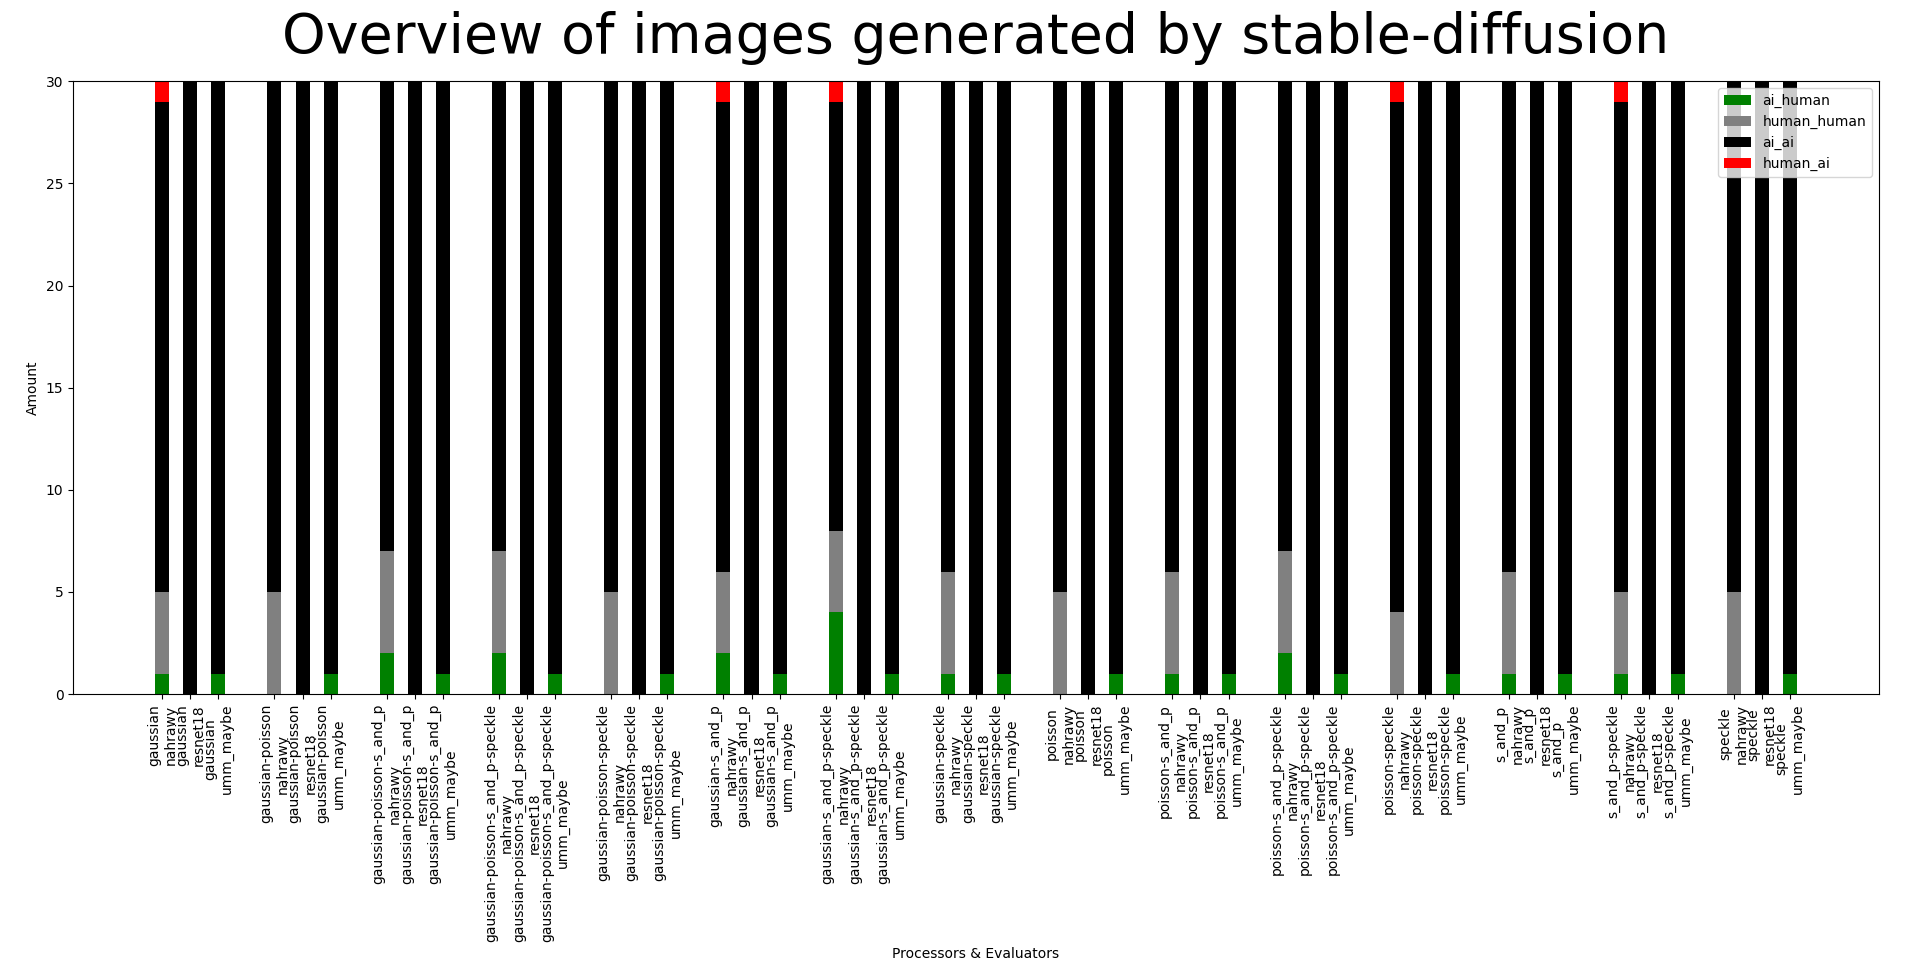
\includegraphics[width=\linewidth]{images/stable-diffusion.png}
	\caption{Stable Diffusion with different processors and nahrawy, resnet18 and umm-maybe as evaluators}
	\label{fig:stable_diffusion}
\end{figure}

\begin{figure}
	\centering
	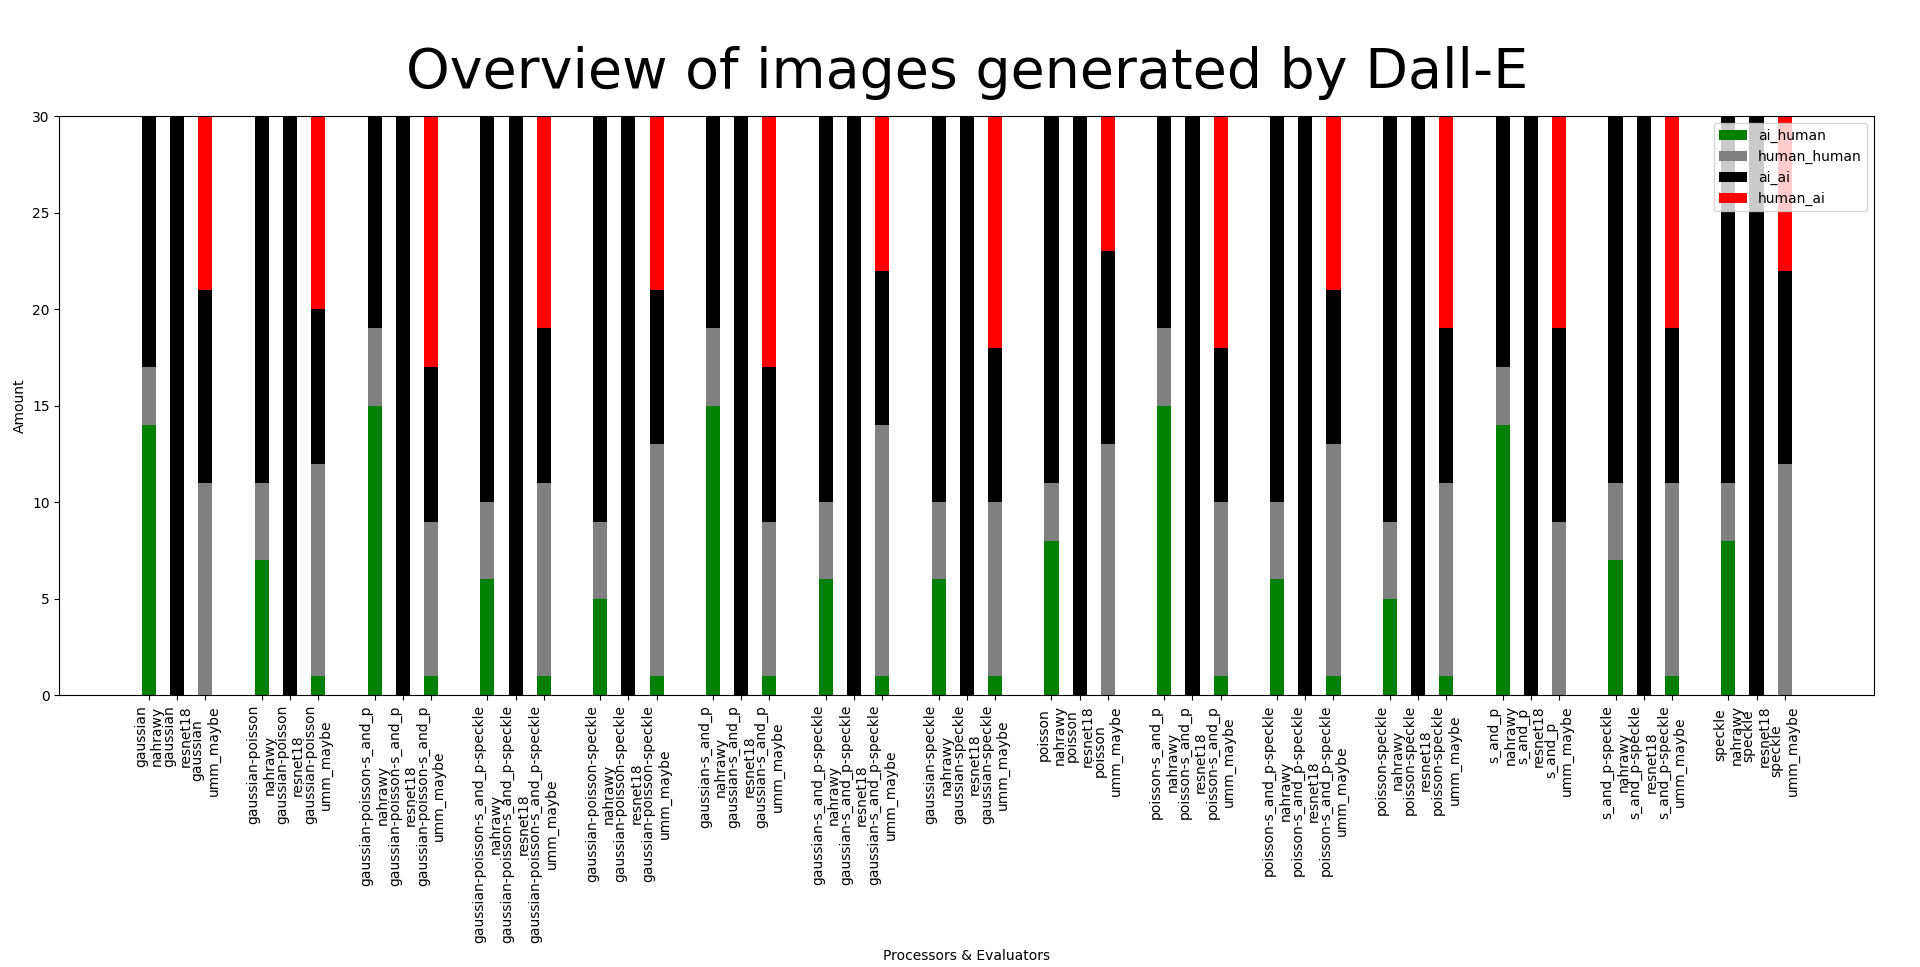
\includegraphics[width=\linewidth]{images/dalle.png}
	\caption{Dall-E with different processors and nahrawy, resnet18 and umm-maybe as evaluators}
	\label{fig:dallE}
\end{figure}


In fig. \ref{fig:gpt2} the text processors are plotted. The colors stay the same and the concept as well, where the left bar is using the radar evaluator and the right one the roberta base one. It is visible that the double-whitespace processor solely has little effect whereas in combination with the typo processor the result rises enormously. This is due to the typo processor since it alone also achieves great results. The radar evaluator only produces only black bars. 
Similar results can be seen in fig. \ref{fig:falcon} where radar just contains black bars and typo as well, as its combination with the roberta base evaluator achieves great results. The difference is that with the falcon generator and the roberta base evaluator in combination, some texts are detected as human made even before processing, which explains the red and grey parts. 

\begin{figure}
	\centering
	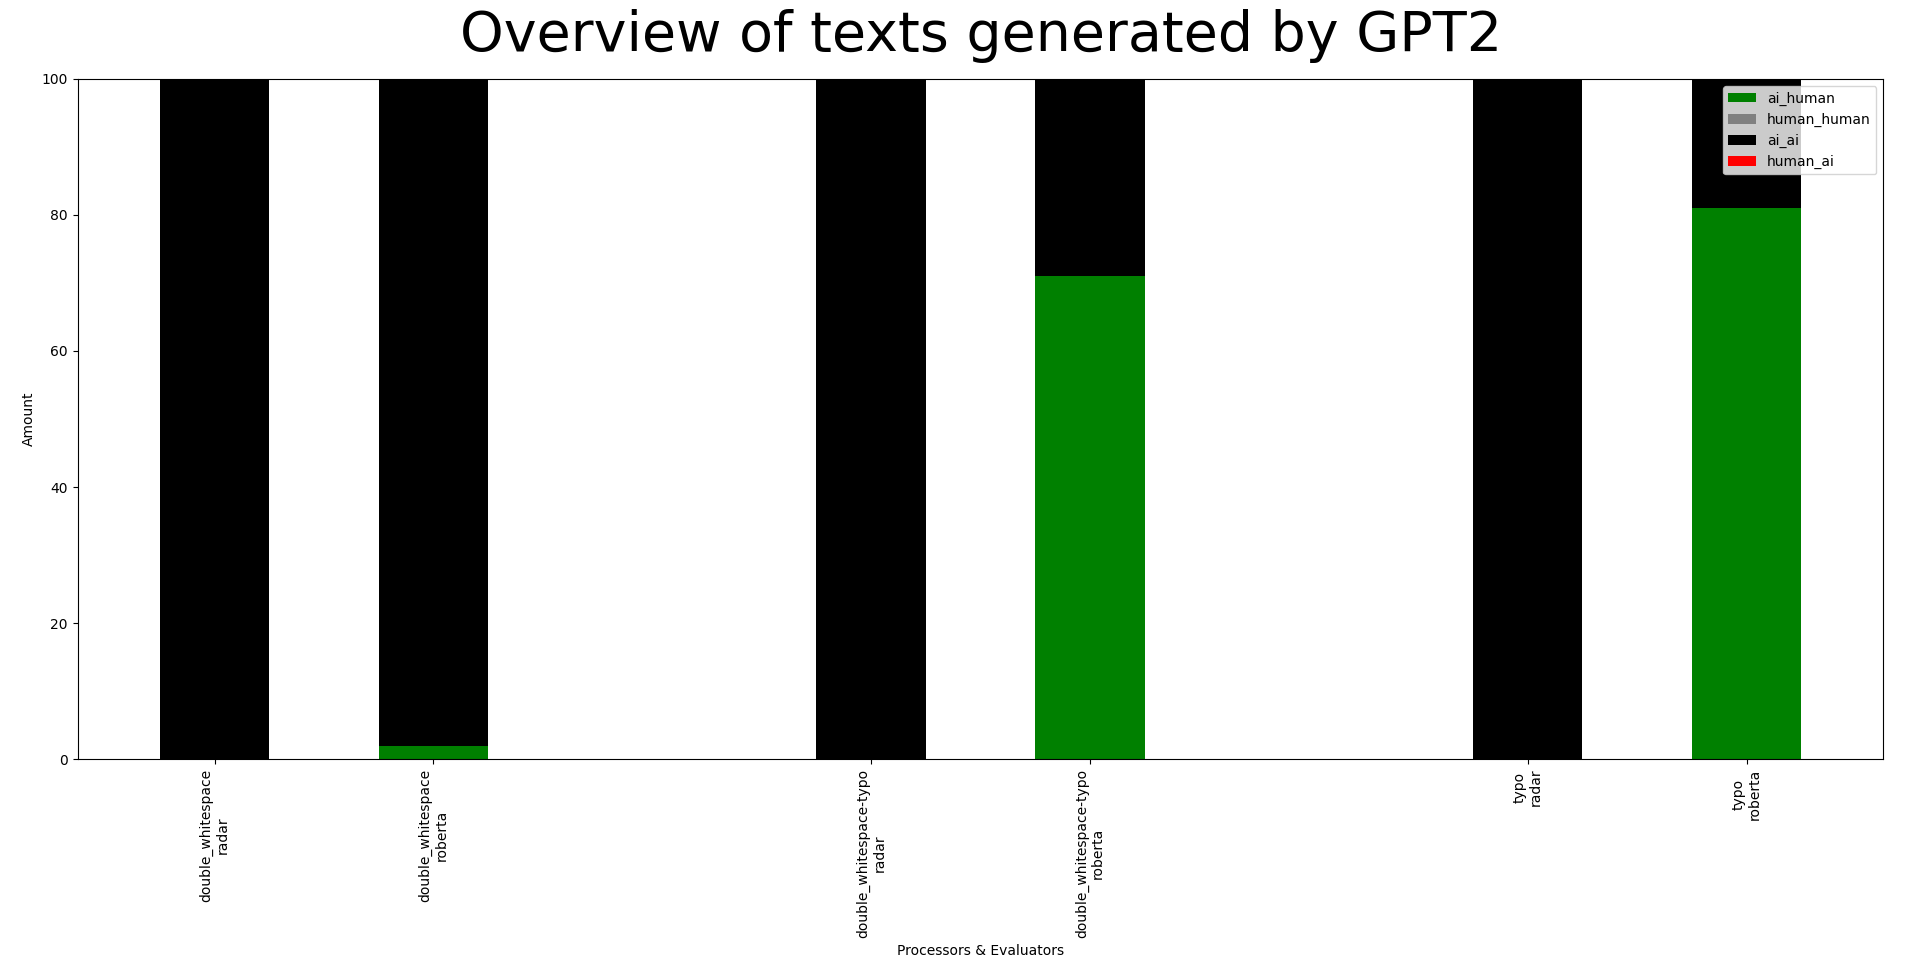
\includegraphics[width=\linewidth]{images/gpt2.png}
	\caption{GPT2 with different processors and nahrawy, resnet18 and umm-maybe as evaluators}
	\label{fig:gpt2}
\end{figure}

\begin{figure}
	\centering
	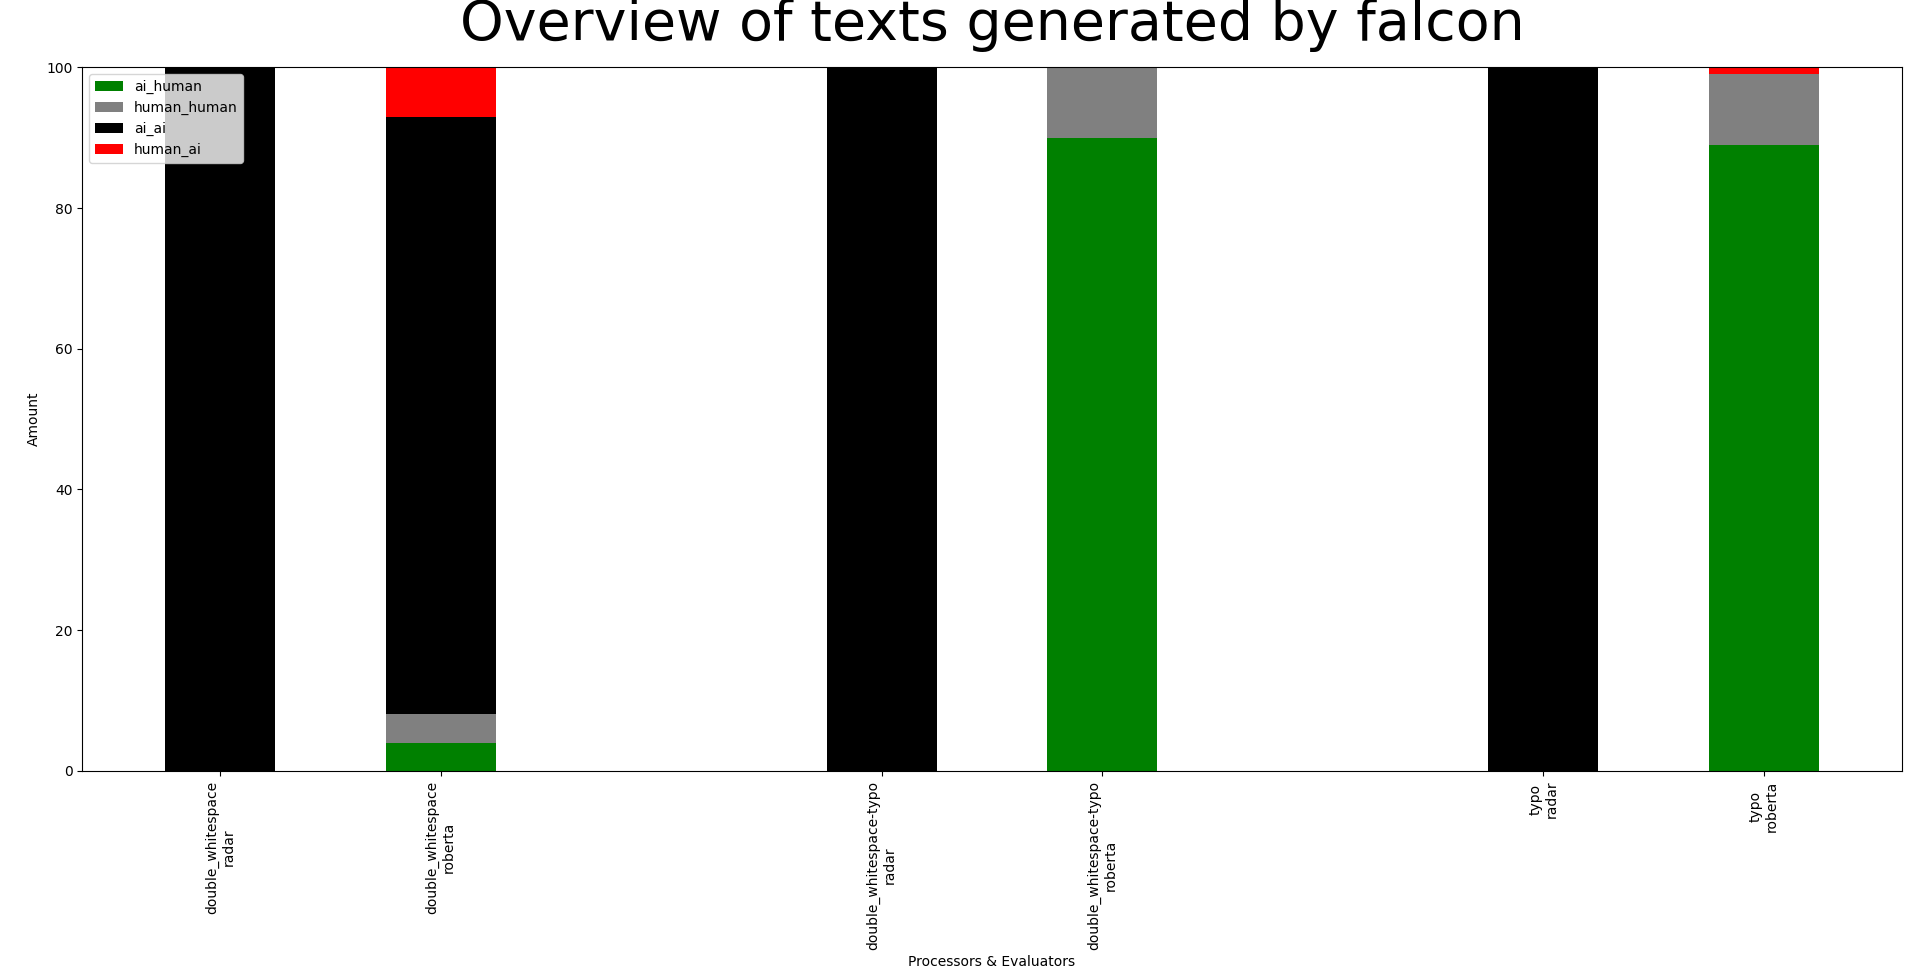
\includegraphics[width=\linewidth]{images/falcon.png}
	\caption{Falcon with different processors and nahrawy, resnet18 and umm-maybe as evaluators}
	\label{fig:falcon}
\end{figure}


To summarize we can say, that the combination between generators and evaluators plays a huge role in the results. In case of the text generators the difference seems minor, but for example the roberta base evaluator detected around ten falcon generated texts as human made in the middle case of fig. \ref{fig:falcon} and after processing as well, which means that if that would not have been the case, we would have a perfect score here. 
This becomes more clear when comparing fig. \ref{fig:stable_diffusion} with fig \ref{fig:dallE} where the importance of the used generators becomes visible. The stable-diffusion generator produces images where it is difficult to fool a detector whereas when using the same processors and detectors, the images of dallE can be processed in a way to fool some detectors.


Another noticeable result is in the usage of different evaluators. In both cases, text and image, we had one evaluator respectively which could not be fooled with any method. These evaluators where so strict, that they would even classify a human made image provided by us as AI-generated.

\section{Conclusion}


\subsubsection*{Acknowledgments}


\bibliography{bibliography}
\bibliographystyle{iclr2024_conference}

\appendix
\section{Appendix}
You may include other additional sections here.

\end{document}
